\chapter{Power Measurement}

\section{Validating RAPL Accuracy}
Starting with the Haswell microarchitecture Intel integrated current measurement into their processor to support power limiting~\cite{Hackenberg_2015_Haswell}.
The associated power metrics for different zones can be measured using the RAPL interface via the linux kernel~\footnote{\url{https://www.kernel.org/doc/html/latest/power/powercap/powercap.html}}.
Schöne et al.~\cite{Schoene_2024_Alder_Lake} tried to validate that RAPL counters on the Alder Lake architecture rely on current measurements, however they found that they are likely using a model.
This is relevant to Sapphire Rapids, since they share the same core microarchitecture Golden Cove.

I validate the accuracy of these counters against an external measurement using roco2 synthetic workload generator.
This software required some patches to run on the current generation of processors.
They are documented in the forked GitHub repository~\footnote{\url{https://github.com/marenz2569/roco2/tree/marenz.hati-config}}.

Each of the displayed workload in~\figref{validate-rapl} were run for \SI{60}{\second} on the cross product of following settings:
\begin{itemize}
    \item Core frequency set to \SI{800}{\MHz}, \SI{1400}{\MHz}, \SI{2000}{\MHz} and \SI{3800}{\MHz} (turbo).
    \item Four settings which represent the execution of the workload on an increasing number of quadrants on the first socket.
    The number of cores used are: \SI{14}{}, \SI{28}{}, \SI{42}{} and \SI{56}{}.
\end{itemize}
The test matrix further included a full idle for each C-state setting (POLL, C1, C1E, C6).
Hyperthreading is disabled and the governor set to \texttt{performance}.
The power metrics were measured through the FIRESTARTER measurement inferface.
This polls the RAPL metrics every \SI{10}{\ms} and discovered the first and last \SI{5}{\second} of each measurement duration.
The external reference measurent of the PDU is exposed via the metricq~\cite{Ilsche_2019_MetricQ} interface of FIRESTARTER~\footnote{\url{https://github.com/marenz2569/firestarter-metric-metricq}} and reports \SI{1}{Sa\per\second}.
The average power draw of the PDU and the RAPL counters is plotted in~\figref{validate-rapl}.
A strong correlation via quadratic fit can be observed, indication that RAPL metrics are being measured.
All measurment points are inside the \SI{1}{\percent} tolerance of the PDU.

\begin{figure}[]
    \centering
    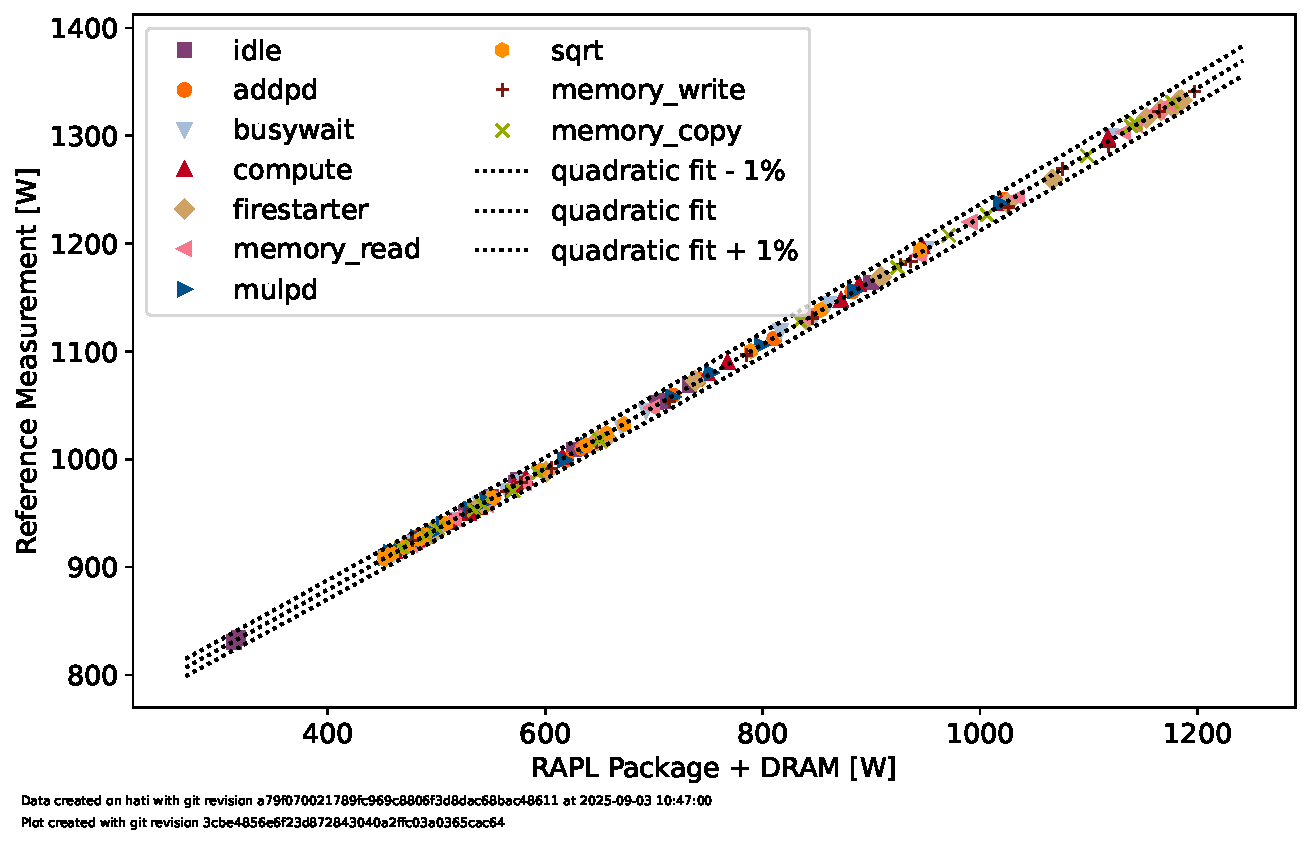
\includegraphics[width=0.8\columnwidth]{fig/rapl-accuracy/rapl-accuracy.pdf}
    \caption{\label{fig:validate-rapl}The roco2 microbenchmark is executed on a varying number of cores with different frequencies.
    The RAPL measurement can be mapped with a quadratic fit to the external reference measurement.}
\end{figure}

\section{RAPL Filters}

\todoms{Influence of the data on the RAPL measurements.}
\todoms{Influence of the measurement time on the RAPL measurements.}
